\subsection{Partie préconditionneur}
La factorisation LU en algèbre linéaire dense est une méthode pour factoriser une matrice $A$ en deux matrices $L$ et $U$.
%
$L$ est une matrice triangulaire inférieure, toutes les valeurs au-dessus de la diagonale sont nulles.
%
Symétriquement, $U$ est une matrice triangulaire supérieure, toutes les valeurs de $U$ en dessous de la diagonale sont nulles.
%
Le principal intérêt de cette factorisation est de trouver $x$ dans les équations du type $Ax=y$.
%
Cette équation est transformée en deux équations $L.x_{tmp}=y$ et $U.x=x_{tmp}$.
%
La méthode utilisée pour résoudre les systèmes composés de matrices triangulaires est triviale.
%
Il suffit de résoudre chaque équation ligne par ligne en commençant par la ligne qui n'a qu'une seule valeur non nulle.
%
Ensuite il faut résoudre la ligne avec deux valeurs non nulles dont une des inconnues provient de la solution précédente, et ainsi de suite jusqu'à la dernière ligne.
%
Il existe du parallélisme à exploiter dans cet algorithme, à chaque fois qu'une inconnue est trouvée, on peux la retirer de chacune des lignes restantes à traiter~\cite{plasma_lu}.



En algèbre linéaire creuse, la factorisation LU d'une matrice $A$ creuse donnera deux matrices triangulaires denses $L$ et $U$.
%
Or, dans le cas d'une matrice d'ordre élevé ($>$ 100 000), ces deux matrices ne peuvent pas tenir en mémoire.
%
C'est pourquoi en algèbre linéaire creuse, on utilise une version altérée de cette factorisation que l'on appelle factorisation incomplète, ou {\em ILU}\footnote{Incomplete LU}, dont le but est de limiter le remplissage de la matrice.
%
L'algorithme ILU est similaire à l'algorithme LU mais le remplissage est limité par des conditions définies par l'algorithme.
%
Ces conditions peuvent être de deux formes, soit en limitant le remplissage avec une valeur seuil (ILUT), soit en limitant le niveau d'interaction entre les lignes de la matrices (ILU(k)).
%
Dans le cas ILU(k), le paramètre k sert à limiter le niveau d'interaction entre les lignes.
%
Avec $k=0$, le motif des matrices $L$ et $U$ reste similaire au motif de la matrice $A$.
%
Le parallélisme exploitable dans l'algorithme ILU est différent de celui exploitable dans l'algorithme LU, il offre la possibilité de factoriser certaines lignes en parallèle et ce parallélisme se représente naturellement sous la forme d'un graphe de tâches (Fig.~\ref{fig:example_3_dag}).
%
Chaque tâche représentant la factorisation d'une ligne de la matrice et les dépendances entre les tâches sont données par le motif de la matrice.
%
En effet, pour factoriser la ligne $i$, nous devons factoriser toutes les lignes $j$ inférieures à $i$ tel que l'entrée $(i,j)$ de la matrice soit non nulle (Fig.~\ref{fig:example_2_matrix}).
%
Donc, à partir du motif des valeurs non-nulles de la matrice, nous pouvons facilement construire le graphe de tâche:
%
la tâche $i$ corresponds à la ligne $i$ de la matrice, la liste des taches prédécesseurs de la tâche $i$ est donnée par l'index de colonne des valeurs non-nulles avant la diagonale dans la ligne $i$ et la liste des tâches successeurs de la tâche $i$ est donnée par l'index de ligne des valeurs non-nulles au-dessous de la diagonale de la colonne $i$ (Algo~\ref{algo:ilu0}).

\begin{figure}[!ht]
     \begin{center}
        \subfigure[Un réservoir à 4 cellules]{%
          \label{fig:example_1_res}
          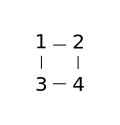
\includegraphics[width=0.32\textwidth]{example_1_res}
        }%
        \subfigure[Une matrice avec 4 cellules]{%
          \label{fig:example_2_matrix}
          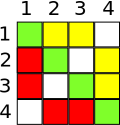
\includegraphics[width=0.32\textwidth]{example_2_matrix}
        }%
        \subfigure[Un DAG à 4 cellules]{%
          \label{fig:example_3_dag}
          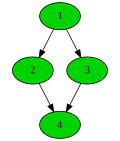
\includegraphics[width=0.32\textwidth]{example_3_dag}
        }%
    \end{center}
    \caption{Trois représentations d'un réservoir. Les éléments en rouge dans la matrice déterminent les dépendances dans le graphe de tâches.}
    \label{fig:exemple_3_dag}
\end{figure}

\begin{algorithm}
  \KwData{$M$ : matrice de dimension $n$}
  \For{$i = 2$ {\bf à} $n$} {
    \For{$k = 1$ {\bf à} $i - 1$ {\bf et} $M_{ik} != 0$} {
      $M_{ik} = M_{ik} / M_{kk}$ \\
      \For{$j = k + 1$ {\bf à} $n$ {\bf et} $M_{ij} != 0$} {
        $M_{ij} = M_{ij} - M_{ik}M_{kj}$ \\
      }
    }
  }
  \caption{Factorisation ILU(0) sur place.}
  \label{algo:ilu0}
\end{algorithm}


En résumé, le parallélisme de l'algorithme ILU peut se représenter sous la forme d'un graphe de tâches.
%
Chaque tâche représentant la factorisation d'une ligne... ce qui est bien petit.
%
En fait, la plupart des runtimes mettront plus de temps à ordonnancer la tâche que la tâche mettra à factoriser une ligne.


Les problèmes rencontrés pour paralléliser la factorisation incomplète d'une matrice creuse, ainsi que les résolutions triangulaires associées, sont des problèmes qui représentent bien la difficulté que l'on peut rencontrer avec une parallélisation à grain fin.
%
La description à grain fin de ces algorithmes est naturelle, mais en pratique, une simple parallélisation utilisant Intel TBB ou OpenMP ne donnera pas de bonnes performances à cause du faible coût de calcul d'une tâche.
%
On appelle cela le problème de granularité.
%
Pour résoudre ce problème, les tâches doivent devenir plus grosses, nous devons factoriser plusieurs lignes à l'intérieur d'une tâche.
%
Mais le choix de ces lignes n'est pas trivial, il faut limiter l'impact sur le parallélisme et ne pas changer le résultat final.
%
Une méthode générique a été développée durant la thèse et sera expliquée plus loin dans ce document.


Il existe des travaux de recherche dont le but est aussi d'exploiter le parallélisme de l'algorithme ILU.
%
En changeant la numérotation des cellules, on peux modifier la structure de la matrice ce qui aura pour effet de changer la factorisation.
%
Une renumérotation rouge-noir permet de factoriser parallèlement la moitié des lignes de la matrice dans un premier temps, puis la seconde moitié des lignes dans un second temps.
%
Cette technique offre énormément de parallélisme mais aura un impact négatif sur la convergence\cite{red_black_ilu}.
%
Plus récemment, une autre méthode a été développée permettant de factoriser tous les éléments de la matrice en parallèle.
%
L'opération de factorisation parallèle est appelé {\em sweep} et est effectuée plusieurs fois\cite{chow2014fine}.
%
En moyenne 3 sweeps suffisent à obtenir un résultat proche de la factorisation incomplète.
%
La convergence n'est donc que faiblement dégradée, mais il faut prendre en compte que 3 sweeps ont été nécessaires et il a donc fallu faire 3 fois plus d'opérations qu'une factorisation ILU.

%   (-_-)   %
\begin{figure}[!ht]
     \begin{center}
        \subfigure[Exemple de graphe de tâche obtenu avec une numérotation naturelle.]{%
          \label{fig:DAG_natural}
          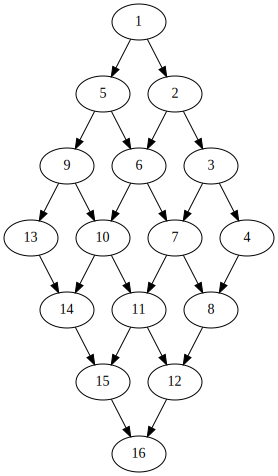
\includegraphics[width=0.33\textwidth]{DAG_natural}
        }%
        \subfigure[Exemple de graphe de tâche obtenu avec une numérotation rouge-noire.]{%
          \label{fig:DAG_redblack}
          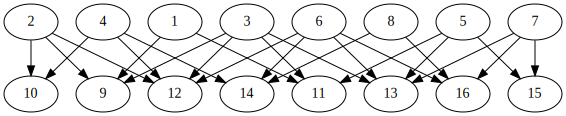
\includegraphics[width=0.66\textwidth]{DAG_redblack}
        }%
    \end{center}
    \caption{Différence de parallélisme en fonction de la numérotation choisie.}
    \label{fig:DAG_ordering}
\end{figure}
